\chapter*{Appendix A: Feature importance on Shapley plots}
\label{appendix:A}

\renewcommand{\thefigure}{A.\arabic{figure}} 
\setcounter{figure}{0} % Reset figure counter

\begin{figure}[h]
    \centering
    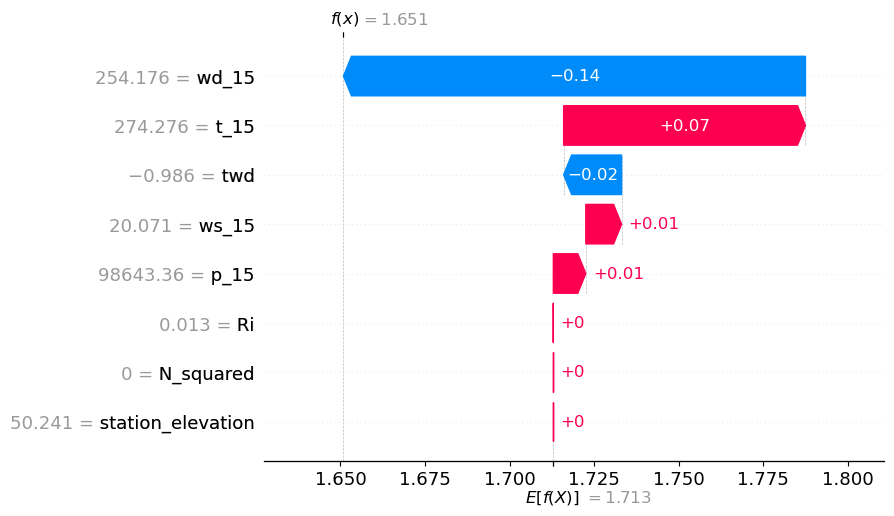
\includegraphics[scale = 0.6]{Figures/shap_plots/waterfall_plot.png}
    \caption[Feature importance for a single observation of a neural network.]{Feature importance of a neural network with model architecture as described in Table \ref{table:gridSearchHyperparamters} and data as described in Table \ref{table:trainDataExample}. In this specific instance the wind direction ($wd_{15}$) has the highest negative influence and the temperature has the highest positive influence. Elevation data is excluded when working with Shapley values, as the contribution of each elevation point is very low and there are very many of them. To see their influence on the model output see Table \ref{table:results}.}
    \label{fig:ShapleyWaterfall}
\end{figure}

\begin{figure}
    \centering
    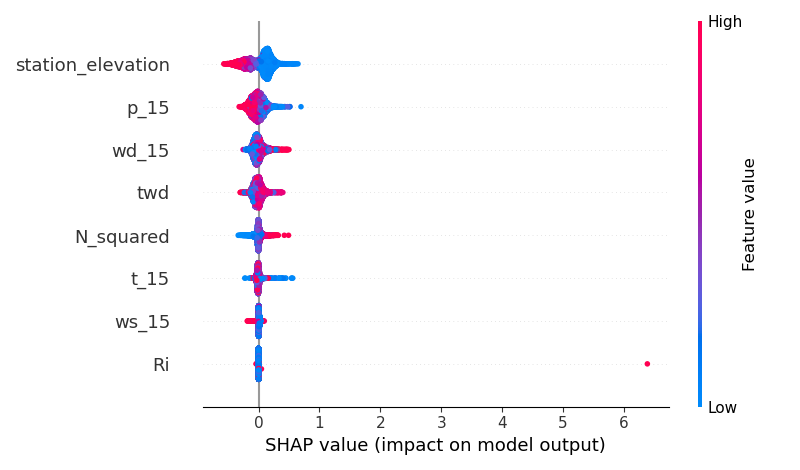
\includegraphics[scale = 0.6]{Figures/shap_plots/summary_plot.png}
    \caption[Summary feature importance of a neural network.]{Feature importance of a neural network with model architecture as described in Table \ref{table:gridSearchHyperparamters} and data as described in Table \ref{table:trainDataExample}. We can see that generally multiple factors influence the prediction, with the station elevation being highly influential. There is seemingly one outlier for the Richardson number, which usually has very little influence. Elevation data is excluded when working with Shapley values, as the contribution of each elevation point is very low and there are very many of them. To see their influence on the model output see Table \ref{table:results}.}
    %\label{fig:ShapleySummary}
\end{figure}

\begin{figure}
    \centering
    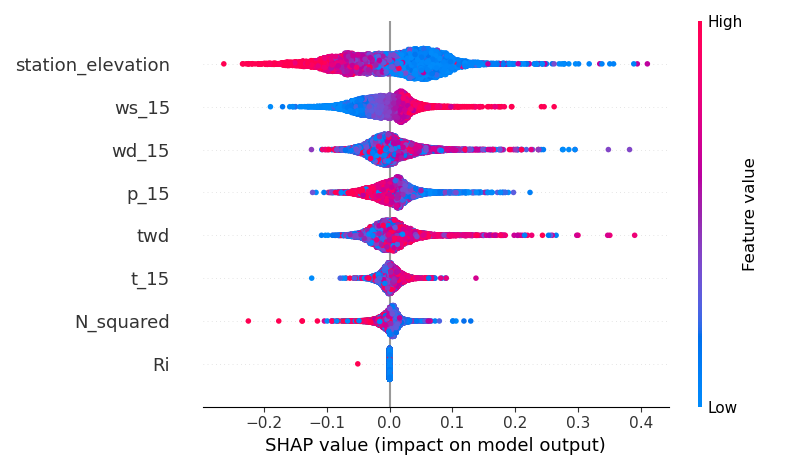
\includegraphics[scale = 0.6]{Figures/shap_plots/summary_plot_190924_.png}
    \caption[Summary feature importance of a neural network using a larger distribution of data.]{Feature importance of a neural network with model architecture as described in Table \ref{table:gridSearchHyperparamters} and data as described in Table \ref{table:trainDataExample}. Generally multiple factors influence the prediction, with the station elevation being highly influential. Elevation data is excluded when working with Shapley values, as the contribution of each elevation. In contrast to Figure (\ref{fig:ShapleySummary}), the distribution doesn't have as extreme outliers. This means that more details can be seen in the figure. The X-axis shows the influence of feature values on the model. The color gradient shows the value of each feature. As an example, there is a very red value for station elevation (top line, all the way to the left). This means that in this instance, the station elevation contributed around -0.25 to the final output and that the station had an elevation significantly above average.}
    %\label{fig:ShapleySummary2}
\end{figure}

\begin{figure}
    \centering
    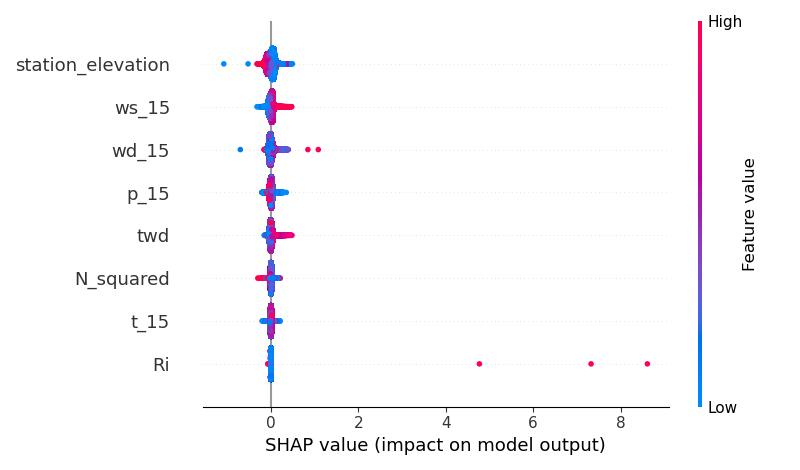
\includegraphics[scale = 0.6]{Figures/shap_plots/summary_plot_190924_full_10ms.png}
    \caption[Summary feature importance of a neural network using entire dataset.]{Feature importance of a neural network with model architecture as described in Table \ref{table:gridSearchHyperparamters} and data as described in Table \ref{table:trainDataExample}. The distribution seems to be the same as before, discounting the outliers.}
    \label{fig:ShapleySummary3}
\end{figure}

\begin{figure}
    \centering
    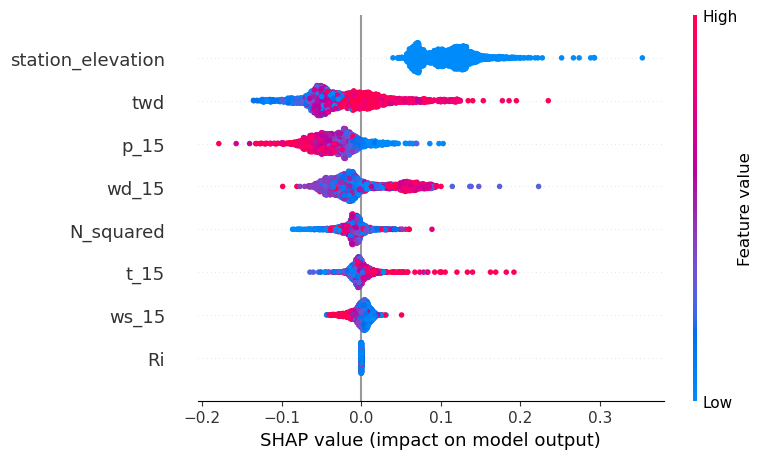
\includegraphics[scale = 0.6]{Figures/shap_plots/summary_plot_31572.png}
    \caption[Summary feature importance of a neural network only looking at AWS at Akrafjall.]{Feature importance of a neural network with model architecture as described in Table \ref{table:gridSearchHyperparamters} and data as described in Table \ref{table:trainDataExample}. This plot only looks at datapoints from Akrafjall. This seems to show the same distribution as previous summary plots. Station elevation is influential and Richardson number has no impact.}
    \label{fig:ShapleySummaryAkrafjall}
\end{figure}

\begin{figure}
    \centering
    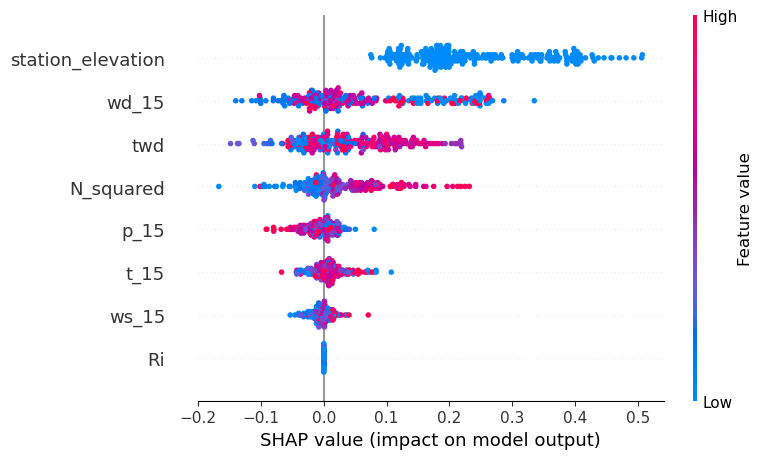
\includegraphics[scale = 0.6]{Figures/shap_plots/summary_plot_35553.png}
    \caption[Summary feature importance of a neural network only looking at AWS at Almannaskarð.]{Feature importance of a neural network with model architecture as described in Table \ref{table:gridSearchHyperparamters} and data as described in Table \ref{table:trainDataExample}. This plot only looks at datapoints from Almannaskarð. This seems to show the same distribution as previous summary plots. Station elevation is influential and Richardson number has no impact.}
    \label{fig:ShapleySummaryAlmannaskarð}
\end{figure}

\begin{figure}
    \centering
    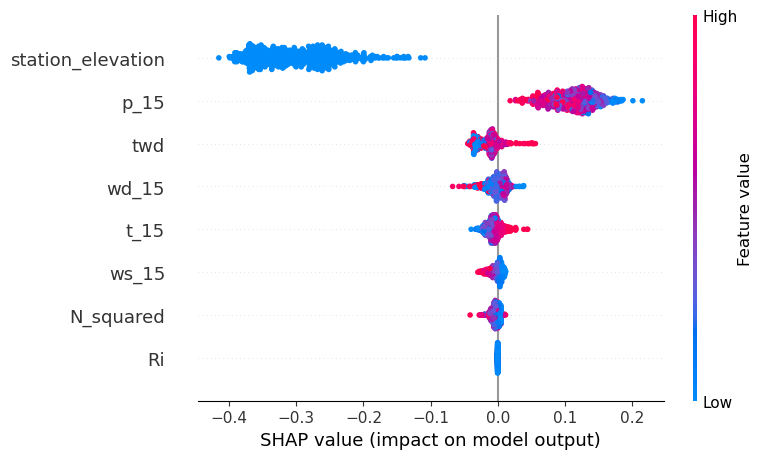
\includegraphics[scale = 0.6]{Figures/shap_plots/summary_plot_6745.png}
    \caption[Summary feature importance of a neural network only looking at AWS at Ásgarðsfjall.]{Feature importance of a neural network with model architecture as described in Table \ref{table:gridSearchHyperparamters} and data as described in Table \ref{table:trainDataExample}. This plot only looks at datapoints from Ásgarðsfjall. This seems to show the same distribution as previous summary plots. Station elevation is influential and Richardson number has no impact.}
    \label{fig:ShapleySummaryAsgarðsfjall}
\end{figure}

\begin{figure}
    \centering
    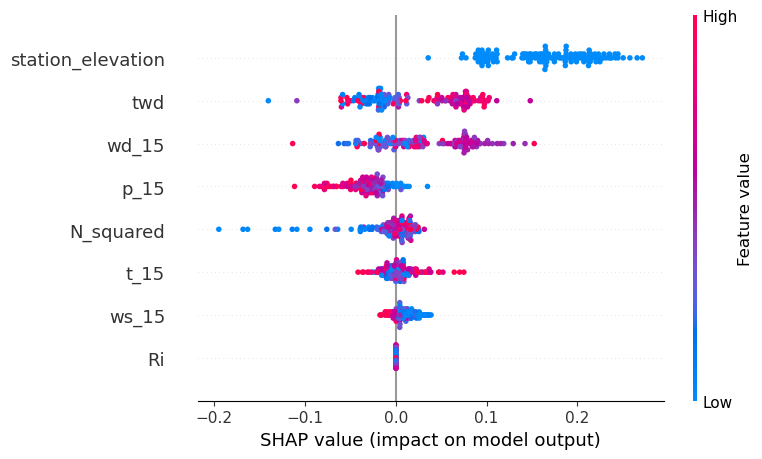
\includegraphics[scale = 0.6]{Figures/shap_plots/summary_plot_1470.png}
    \caption[Summary feature importance of a neural network only looking at AWS at Háahlíð.]{Feature importance of a neural network with model architecture as described in Table \ref{table:gridSearchHyperparamters} and data as described in Table \ref{table:trainDataExample}. This plot only looks at datapoints from Háahlíð. This seems to show the same distribution as previous summary plots. Station elevation is influential and Richardson number has no impact.}
    \label{fig:ShapleySummaryHaahlid}
\end{figure}

\begin{figure}
    \centering
    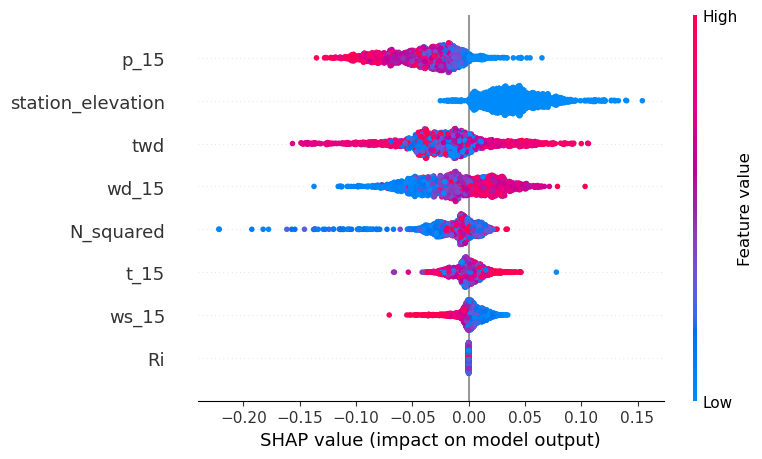
\includegraphics[scale = 0.6]{Figures/shap_plots/summary_plot_1350.png}
    \caption[Summary feature importance of a neural network only looking at AWS at Keflavíkurflugvöllur.]{Feature importance of a neural network with model architecture as described in Table \ref{table:gridSearchHyperparamters} and data as described in Table \ref{table:trainDataExample}. This plot only looks at datapoints from Keflavíkurflugvöllur. This seems to show the same distribution as previous summary plots. Station elevation is influential and Richardson number has no impact.}
    \label{fig:ShapleySummaryKeflavikurflugvollur}
\end{figure}